%!TEX root = ../template.tex
%%%%%%%%%%%%%%%%%%%%%%%%%%%%%%%%%%%%%%%%%%%%%%%%%%%%%%%%%%%%%%%%%%%
%% chapter1.tex
%% NOVA thesis document file
%%
%% Chapter with introduciton


\chapter{Design and Implementation}
\label{cha:design_and_implementation}

The design process adopted was an iterative design approach to build iteratively the solution according to the users' acceptance and feedback retrieved by users test in each iteration. Throughout this chapter, it is detailed all design and implementation decisions considered in order to reach the final prototype.

\section{Sketching}
\label{sec:sketching}

Before starting the development of the interface prototypes which were tested with users, it was performed some sketches in order to organize and explore ideas to tackle the existing usability problems. The most important to reach in the final of this phase was not a functional or complete interface, but some practical ideas that could be applied in the following prototypes.

Considering the extensive list of problems identified, prioritization was an important aspect taken into account throughout all design phases. The first problem explored was the difficulty to comprehend what is the database query purpose.

In the existing interface, users do not have a unique and clear view that facilitates the comprehension of what data could be fetched from the database through the query presented. As illustrated in Figure \ref{fig:example_of_query_representation}, the user can only see some components of the query at a time, due to the usage of tabs to individualize each type of query components. In addition, as can be observed in Figure \ref{fig:ss_existing_layout}, when users open the query, only the query output preview was shown. That was considered a problem in the analysis of the interface for two different points of view:

\begin{itemize}
    \item When the existing interface was tested with users who do not usually use the Platform, they do not easily find out the existence of the tabs and tried to perceive the query purpose only observing the data preview. Besides not being an effective understanding technique, it can be even more difficult when the output contains several columns;
    \item The users accustomed to this data tool revealed that is cumbersome to open and navigate between tabs in order to understand the query.
\end{itemize}

\begin{figure}[tb]
    \centering
    \subcaptionbox{Starting point (only the result is visible)\label{fig:ss_existing_layout}}%
      {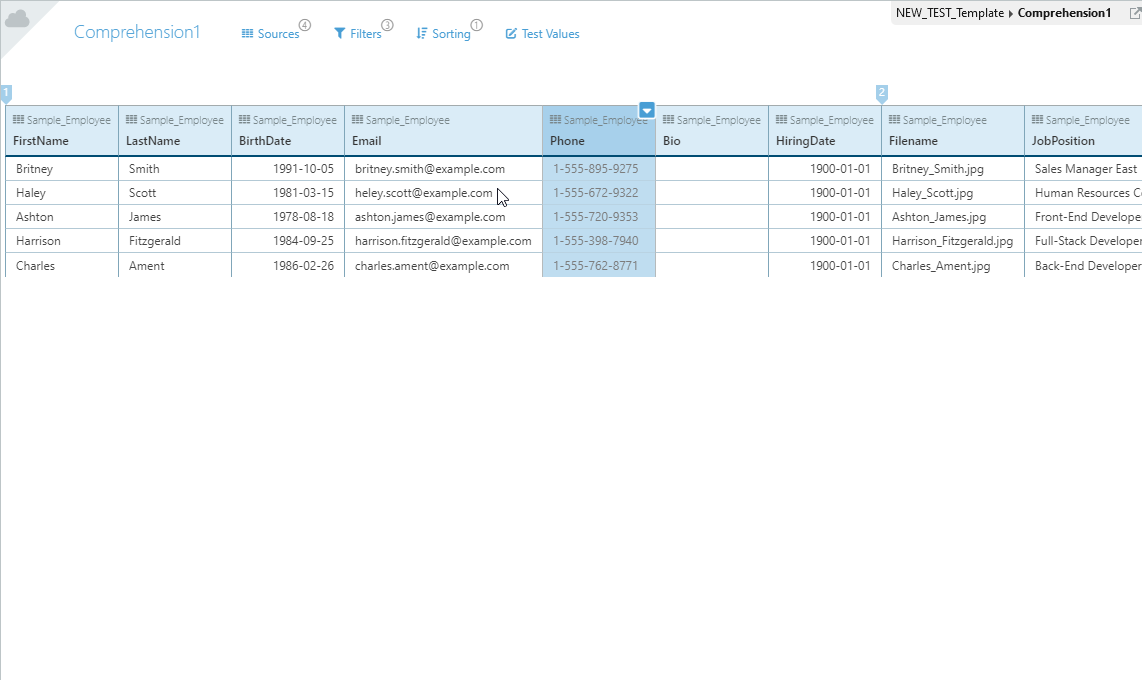
\includegraphics[width=0.5\linewidth]{ss-existing-layout}}%
    \subcaptionbox{Sources Tab\label{fig:ss_existing_layout_sources}}%
      {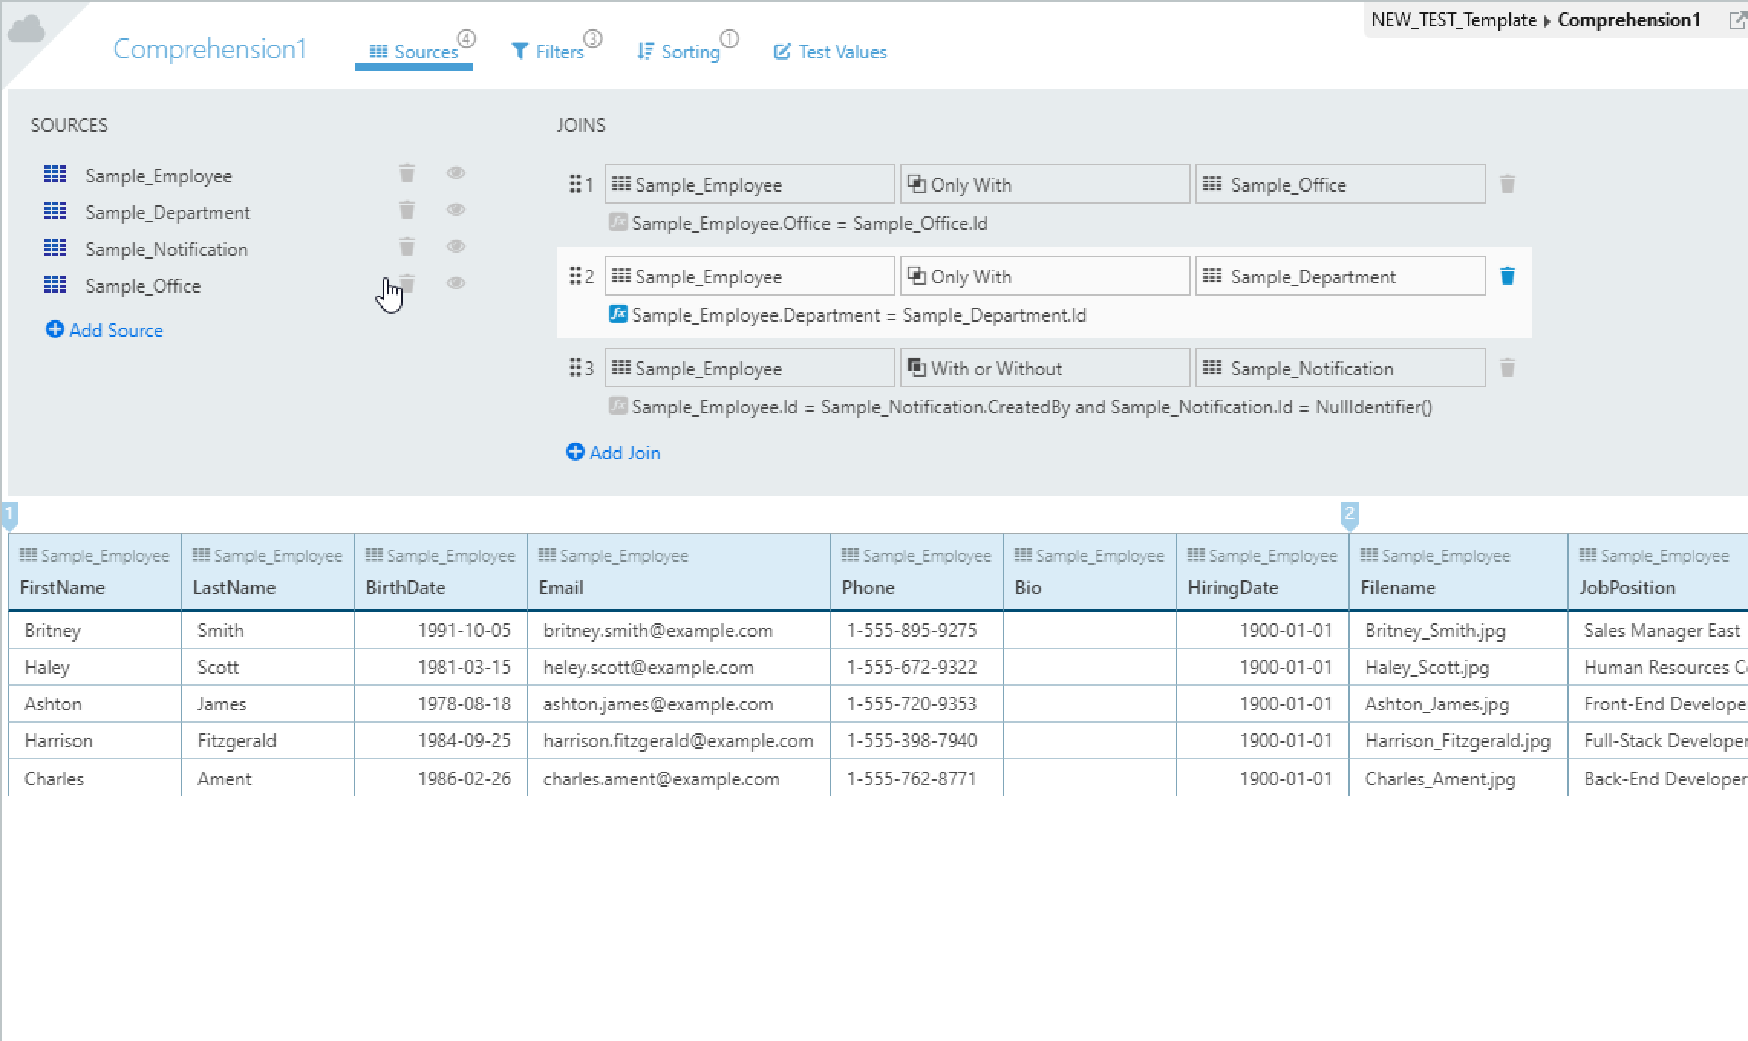
\includegraphics[width=0.5\linewidth]{ss-existing-layout-sources}}%
      \\
    \subcaptionbox{Filters Tab\label{fig:ss_existing_layout_filters}}%
    {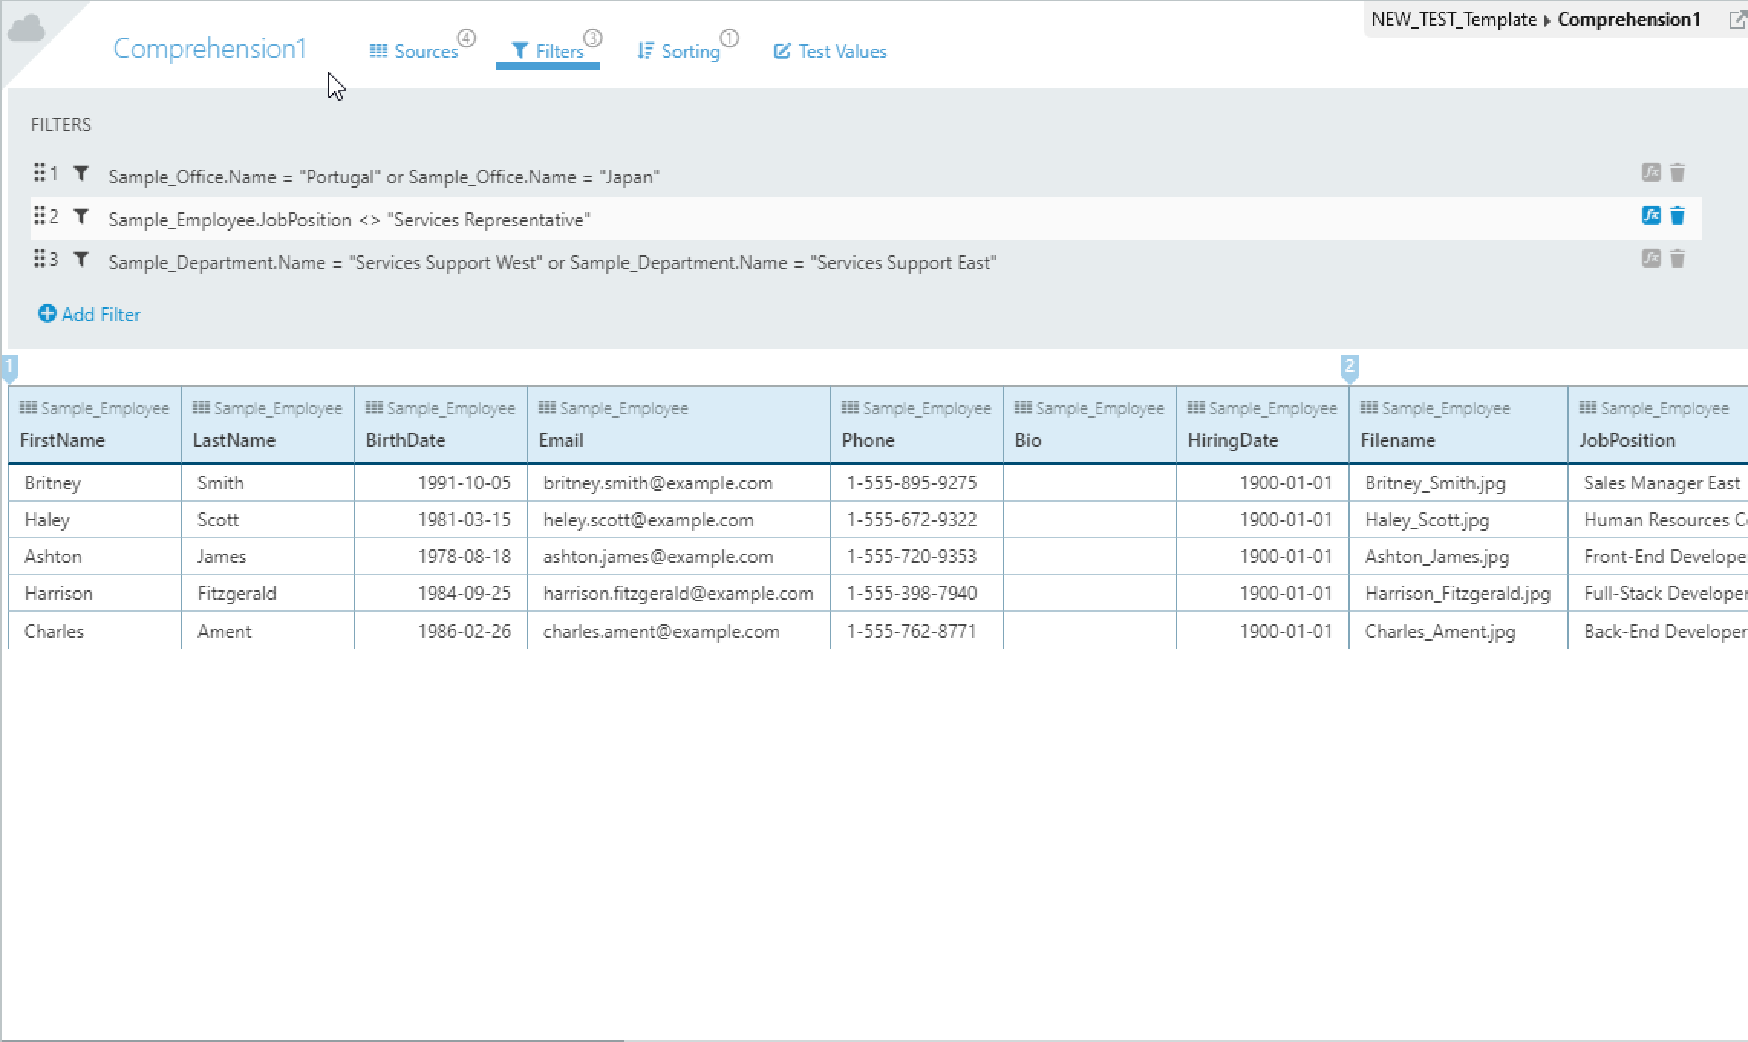
\includegraphics[width=0.5\linewidth]{ss-existing-layout-filters}}%
  \subcaptionbox{Sorting Tab\label{fig:ss_existing_layout_sorting}}%
    {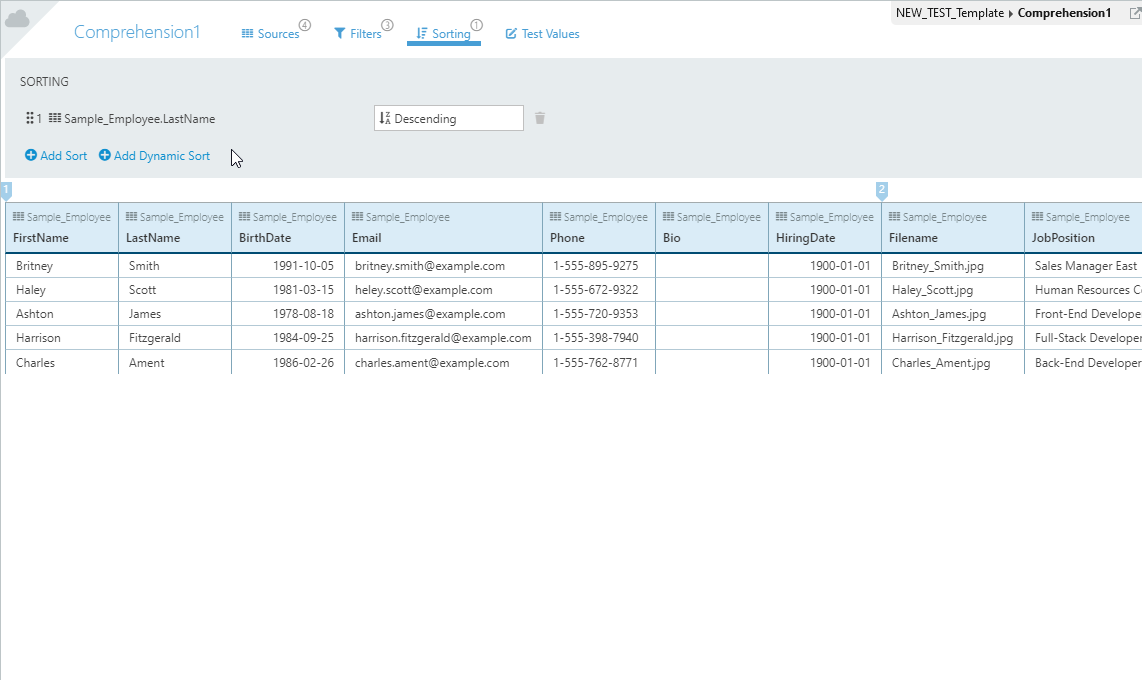
\includegraphics[width=0.5\linewidth]{ss-existing-layout-sorting}}%
  \caption{Example of a database query representation through the existing visual interface.}
    \label{fig:example_of_query_representation}
\end{figure}

Therefore, the designing of a new general layout where it is possible to view the most important query components at once was considered a major requirement. A solid improvement regarding that, could optimize not only the time and effort required to comprehend queries but also to formulate them, since all information is more visible and accessible.

There was also a concern to build a layout that does not compromise the system usability for more complex cases, such as queries that contain a relevant number of entities or conditions.

Accordingly, some wireframes were sketched in order to percept how the query components could be jointly combined in a unique view. Figure \ref{fig:sketch_wireframes} illustrates the two options elected from multiple approaches explored.

In both options, there are two principal areas in the interface as it was before: the query editor area and the preview of the query result. However, it was explored two new manners to display all information of editors jointly with the query result preview. In \nameref{fig:sketch_wireframe_a}, the sub-editors remain in the top area and the query result preview below. The \nameref{fig:sketch_wireframe_b} illustrates another possibility sketched where all editors are presented on the left side of the screen and the visualization of the results are presented on the right side.

\begin{figure}[tb]
  \centering
  \subcaptionbox{Option A\label{fig:sketch_wireframe_a}}%
    {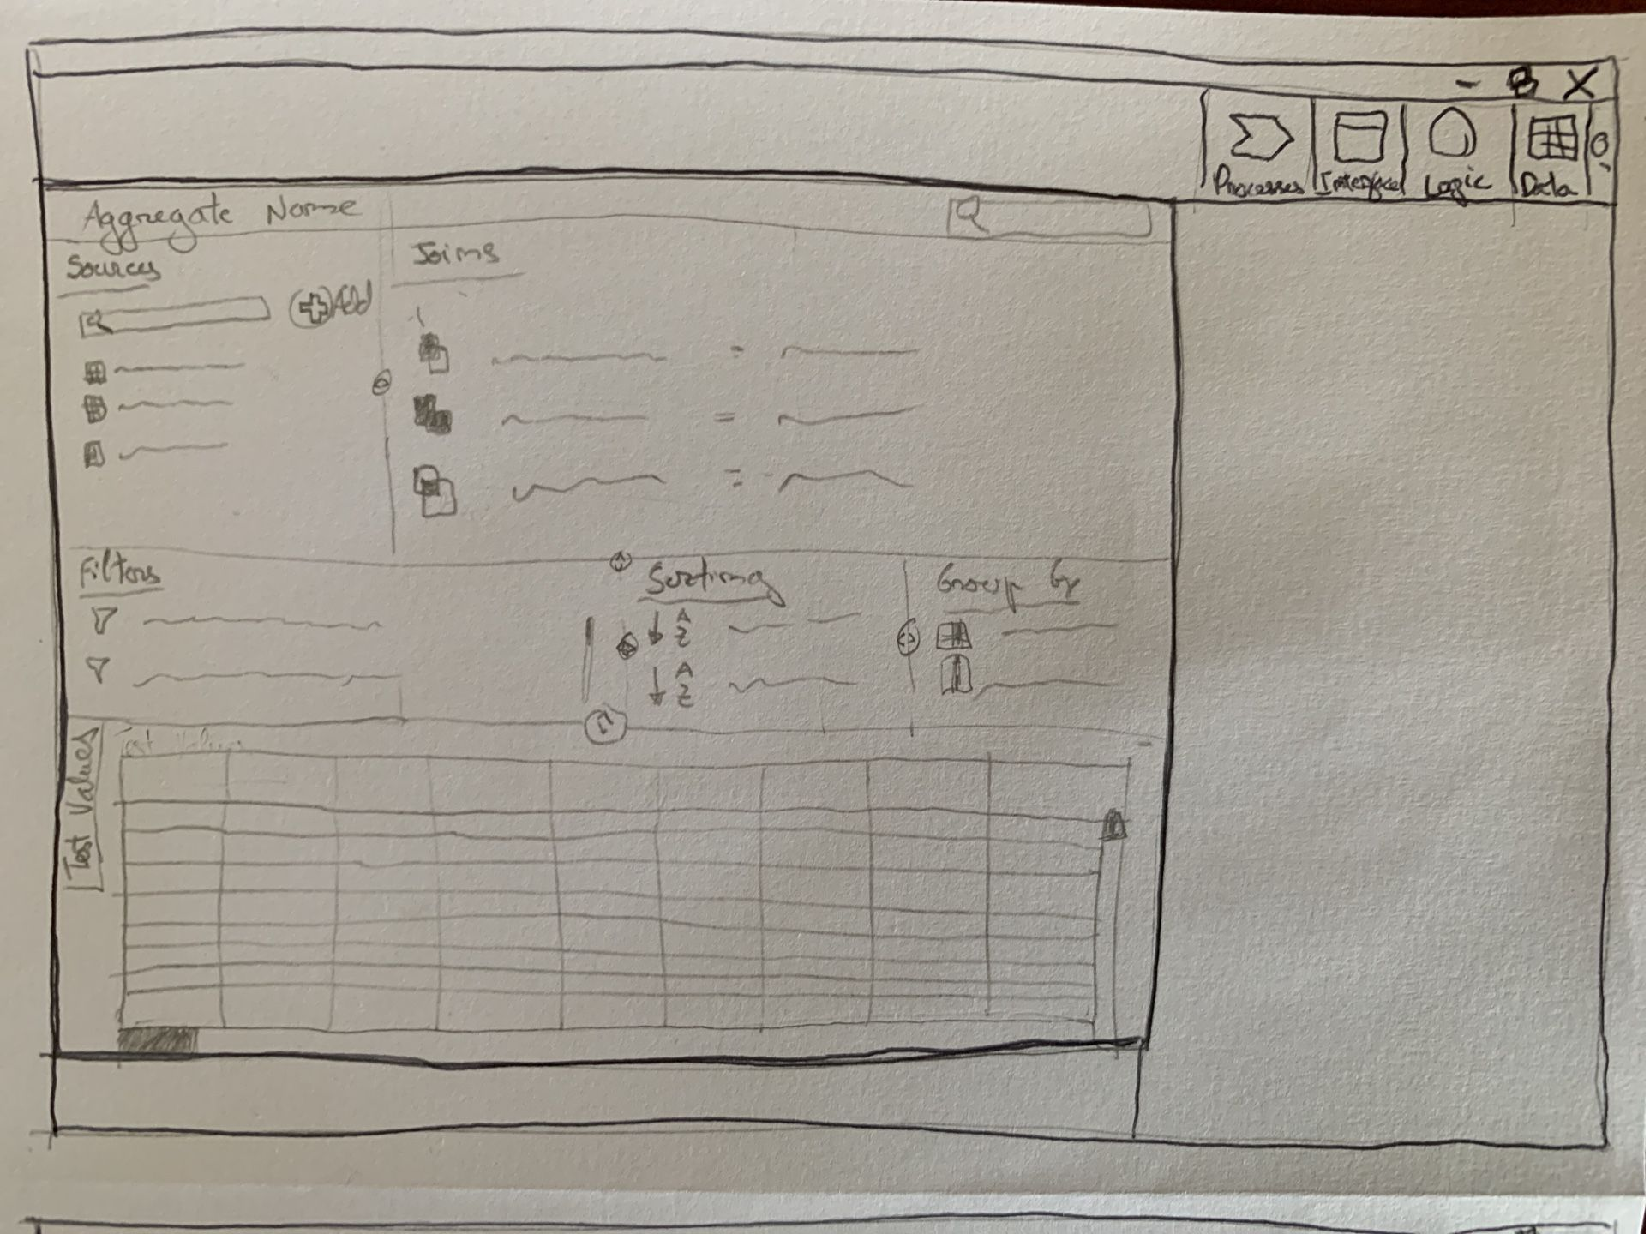
\includegraphics[width=0.5\linewidth]{sketch-wireframe-a}}%
  \subcaptionbox{Option B\label{fig:sketch_wireframe_b}}%
  {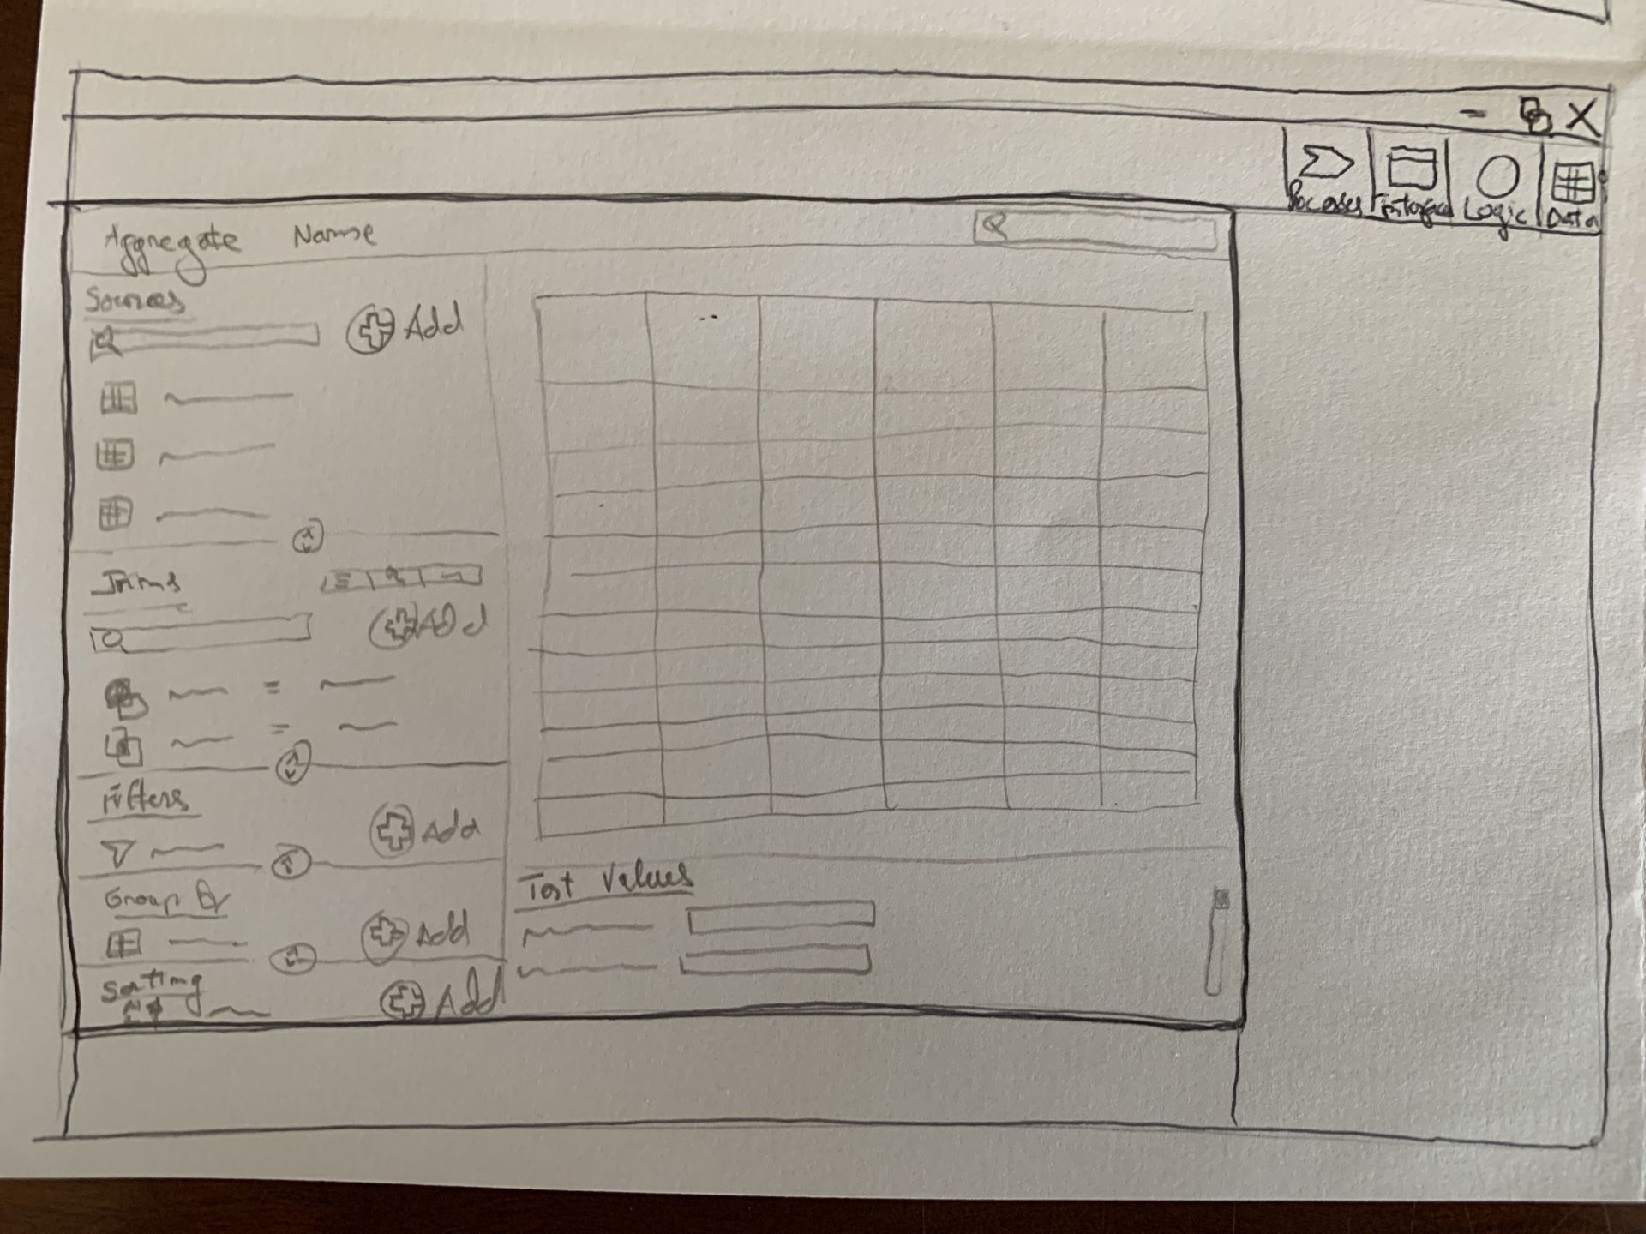
\includegraphics[width=0.5\linewidth]{sketch-wireframe-b}}%
\caption{Interface layout sketches.}
  \label{fig:sketch_wireframes}
\end{figure}

Regardless of the option, the layouts presented have in a single view the most important aspects to understand what query is built.

Beyond the disposition of the different interface views and components, other features were sketched in order to think more about it and structure concrete ideas to implement it.

The existing interface has no mechanism that allows the user to easily find the data of an entity or attribute. The attributes included in the query were not represented in any region of the interface beyond the query result table. Thereby, the unique way to find out the attribute is looking for in each table header, using the horizontal scroll, until the intended attribute is found. That process is cumbersome and slow, so that there was sketched an alternative that includes the attributes in the sources view. Consequently, users can click on attributes and the attribute will be highlighted automatically in the query result preview, as illustrated in Figure \ref{fig:sketchAttributeSearch}. Also, the idea of a search engine was considered, so that users can search for an entity or attribute faster.

\begin{figure}[htbp]
	\centering
	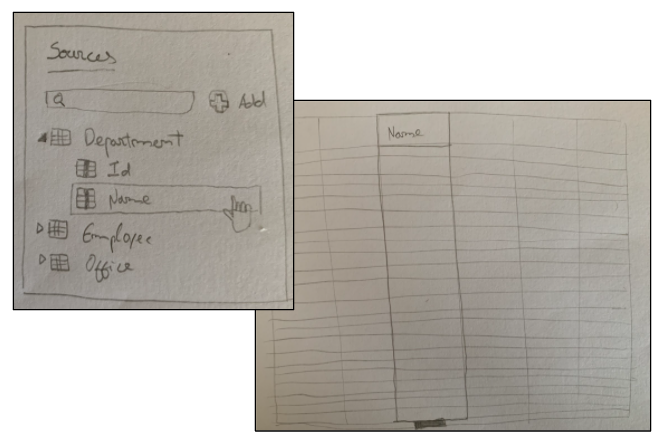
\includegraphics[height=2.5in]{sketch-attribute-search}
	\caption{Searching for an attribute data on the query output preview.}
	\label{fig:sketchAttributeSearch}
\end{figure}

Furthermore, different approaches more compact and functional were explored to display the joins used in the query. Figure \ref{fig:sketchJoins} shows the idea sketched to represent joins in three different lists: a simple list of all join operations inside the query, and two other ones aggregated by the entities involved by the join kind.

\begin{figure}[tb]
  \centering
  \subcaptionbox{Joins flat list\label{fig:sketch-joins-list}}%
    {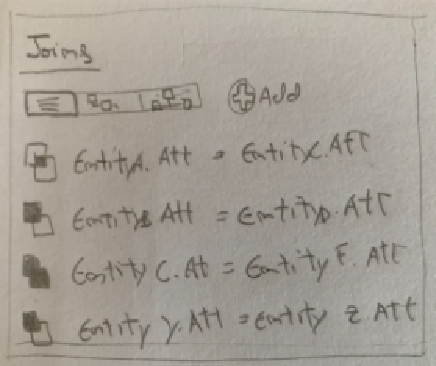
\includegraphics[width=0.3\linewidth]{sketch-joins-list}}%
  \subcaptionbox{Joins associated to each entity\label{fig:sketch-joins-by-entity}}%
  {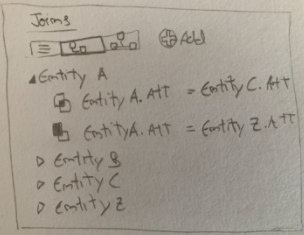
\includegraphics[width=0.3\linewidth]{sketch-joins-by-entity}}%
  \subcaptionbox{Joins by each join kind\label{fig:sketch-joins-by-kind}}%
  {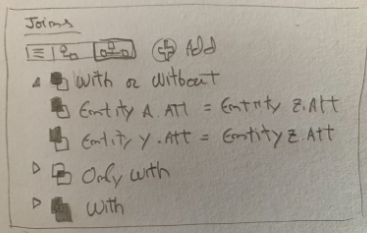
\includegraphics[width=0.3\linewidth]{sketch-joins-by-kind}}%
\caption{Sketches elaborated to explore other approaches to represent the join operations present in the query.}
  \label{fig:sketchJoins}
\end{figure}

Lastly, it was sketched an idea to accelerate the searching process of a specific element inside the query. Therefore, the sketch represented in Figure \ref{fig:sketchGeneralSearch} demonstrates an idea taken into account to find all references of an entity. This general search could allow users to find entities, joins, filters, or other query elements faster.

\begin{figure}[htbp]
	\centering
	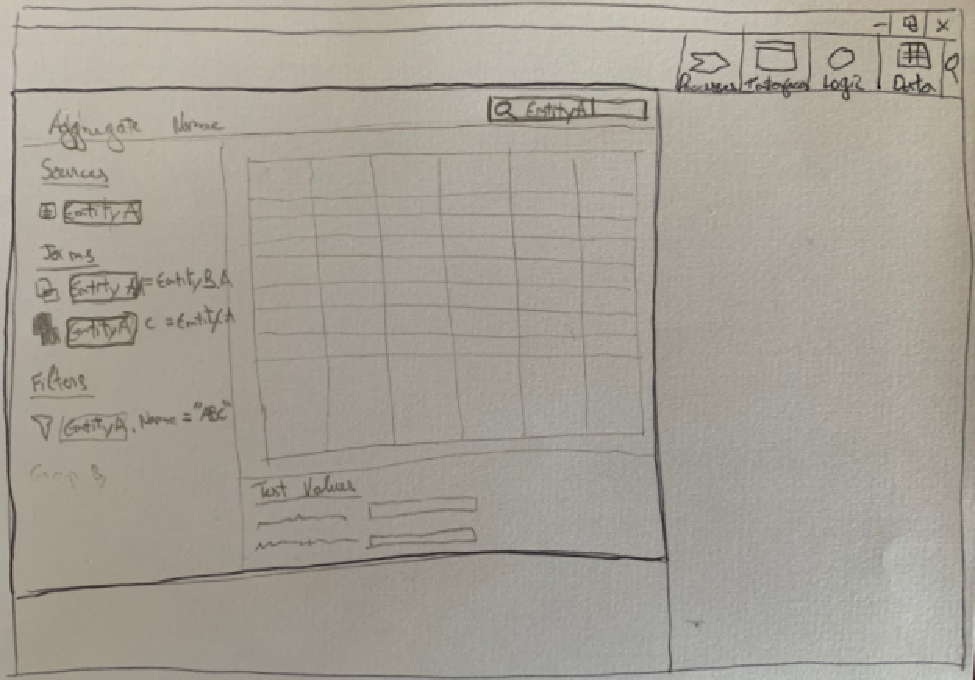
\includegraphics[height=2.5in]{sketch-general-search}
	\caption{Sketch of a general search to allow users to find query elements represented in the interface.}
	\label{fig:sketchGeneralSearch}
\end{figure}

Although the sketched ideas may not be applied to the final prototype since they depend on the whole iterative design process that started afterward, they were important to move the focus from problem definition to solution design.


\section{Paper Prototype}
\label{sec:paper_prototype}
The interactive design process of the solution started in its entirety with the first prototype developed: the paper prototype. The main goal of this phase is the building of a functional prototype implemented in paper using ruler, square, and writing materials, in order to create faster and with a low-risk level a prototype that could be testes by users.

However, due to the COVID-19 pandemic, the prototype was adapted since it was not possible to test the prototype in person. Accordingly, the prototype was scanned and the interactions were configured using the digital product design platform InVision \cite{invision}.
% Do not forget to refer that due to COVID-19 the Paper Prototype was scanned and mounted as a low-fidelity prototype using InVision App.

\subsection{Design}
\label{subsec:paper_prototype_design}
The building process of this low-fidelity prototype started with a design phase where brainstorming took place in order to establish the design priorities for the paper prototype as well as concrete ideas to apply the solutions thought.

\medskip

\textbf{Sub-editors arrangement:}

\medskip

Taking into account the sketches mentioned in the last section, the first question evaluated was which rearrangement of the sub-editors and the result preview views would be implemented in the next phase. In order to take action in this regard, there was a point in the visual query builder background considered. As mentioned in \ref{subsubsec:previous_work}, this querying interface was completely redesigned seven years ago, which had a negative repercussion on users since they were accustomed to the previous interface. Therefore, there was a concern to change the interface without removing the main points that characterize and identifies it. In such a way that users would not feel using a completely new interface but an improved version of the existing one.

Comparing the two options sketched (Figure \ref{fig:sketch_wireframes}) with the existing interface (Figure \ref{fig:example_of_query_representation}), the \nameref{fig:sketch_wireframe_a} is the most similar because the editors area keeps on the top region of the interface and the query result data below. For this reason, this arrangement would be considered in the next phase.

Having chosen where would take place the edition area of the interface, the second aspect taken into consideration was how to organize its sub-editors. This decision was taken bearing in mind what each query aspect represents in the user's mental model when they formulate queries as well as the physical space of the interface they could occupy.

In this regard, it was thought about what are the order of the query elements that arise in user thinking. This reasoning was performed taking into consideration the formulation using \gls{SQL} since one of the main goals is the improvement of the interface experience for users that are proficient in \gls{SQL}. According to the conceptual models presented in \ref{sec:query_conceptual_models}, the first aspect the user thinks, after understanding what data is required, is how to translate them to the query language. In \gls{SQL}, the core statements are presented in the following order:

\begin{enumerate}
  \item \textbf{SELECT: }Indicates which attributes will be selected to be present in the query output table;
  \item \textbf{FROM: }Sets out which entities are used to query data. Thereby, even it is necessary to merge tables, the join operations are specified through that statement;
  \item \textbf{WHERE: }Contains the boolean conditions that would filter the results.
  \item \textbf{ORDER BY: }Specify the criteria to order the data gathered.
\end{enumerate}

In this visual query building tool users do not select attributes because there is an optimizing background task that will inspect where the query is used and only select the attributes that will be used. Therefore, in this system, the information specified through the SELECT statement will not be specified by the user.

However, the three other aspects of the query are clearly specified by users in three different interface areas: Sources, Filters, and Sorting respectively. Accordingly, the arrangement chosen to display these three sub-editors follows this logic. The query edition area were divided into two columns. The left side was elected to represent the sources of the query and the right side lists the filters and sorting criteria.

\medskip

\textbf{New approach to represent sources and joins:}

\medskip

Nevertheless, the way entities and joins were presented in the interface, in the previous sources tab, required to be redesigned from scratch. As can be observed in Figure \ref{fig:ss_existing_layout_sources}, a simple list of the entities used was presented in the left side of the editor area and the joins used to merge them in its right side.

Even though some designs regarding that were elaborated in the sketching phase (Figure \ref{fig:sketchJoins}), it was concluded that the main issues remain:

\begin{itemize}
  \item Difficulty to comprehend faster and with a low-effort what entities were integrated into the query. Being a visual interface, the comprehension of the entities used as source to formulate the query should be easier to understand. However, the potential of the visual interface has not been leveraged, mainly due to the following aspects:
  \begin{itemize} 
    \item \textbf{Textual language overloading: }Not only all join conditions were completely presented in full-textual way, but also the same entity could be written in a repeated way. For example, in the example shown in Figure \ref{fig:ss_existing_layout_sources}, the entity "Sample\_Employee" was presented seven times to indicate that the query uses this entity and this entity was joined with three other entities;
    \item \textbf{Lack of guidance to understand what entities are related to each other: }As the entities and sources are listed in the interface, the design should help users to understand which entities are joined. For instance, if joins were put between the entities involved, it would be simpler to identify if they were merged through a join operation.
  \end{itemize}
\end{itemize}

Therefore, the way entities and joins were listed in the sources tab of the existing interface was reconsidered, since it was intended to create a simpler, intuitive, and compact viewing area.

The idea of a tree view which displays all entities and joins used in the query has emerged to tackle the problem mentioned. Through that approach, it would be possible to reduce the entity repetition and to explicitly perceive which entities have a certain entity been joined.

\medskip

\textbf{Query formulation improvements: }

\medskip

%learnability
Regarding query formulation, there was several users who are not accustomed to the query builder, that had difficulty to discover some functionalities of the system when they tested the existing interface. Thereby, learnability was also considering during the design phase of the first prototype.

As mentioned in \ref{subsec:analysis}, the options to add a new calculated attribute or to apply a group by or an aggregation functions are hidden. These functionalities could be frequently used to apply group data or to add a new column to the output. Therefore, it was concluded that these options should be visible in the sources area. By doing this, not only the options still more visible to the novice users but users have a faster alternative to insert these query components.

%efficiency

Lastly, the distribution of the formulation options (i.e., the buttons or other interface elements that allow users to insert new elements in the query) in the screen was a relevant aspect considered. If the controls of a query component are

The main concern was to put these controls near to the area where the content will be displayed. As an example, if there is an area where entities, joins, and attributes are placed together, the related interaction should be accessible near them. In that way, users do not need to find options in other areas of the interface, keeping the user task on track, avoiding them to lose reasoning context.

That design principle was considered advantageus to reduce the user's working memory overload since they could focus in each part of the query without distractions. Moreover, if the controls are near the time the mouse need to move to them is also less, accelerating the query formulation process.

%Falar da divisão e distribuição do layout
%Falar que tendo em conta o espaço disponível seria necessário encurtar a representação das sources e joins.
%Adicionar fatores diferenciadores para a leitura da query: color highlighting nos filters, melhorar a leitura dos dados na tabela dos resultados, adicionar opções mais visíveis e acessíveis (práticas, rápidas) para adicionar novos attributos.

%Para além disso, foi mais tido em conta a preocupação de colocar numa sub região da interface a maior parte dos controlos mais utilizados, de modo a formulação da query poder ser realizada de forma mais rápida e eficaz, visto que não só se diminui o tempo através da menor distância que o rato tem que percorrer, como também porque o  utilizador vai mantendo o mesmo contexto visual.


\subsection{Implementation}
\label{subsec:paper_prototype_implementation}

After defining design priorities for the current iteration, the paper prototype implementation has launched. In this phase, the pieces of the prototype were built progressively considering the key points presented before and refining some details whenever necessary.

\medskip

\textbf{General layout:}

\medskip

As the reasoning applied in the design phase, the general layout was the first part implemented. 

%Tabela do resultado para cada scenario
%Filtros e sorting de cada scenario

%New sources design
%-Falar sobre as chaves estrangeiras e a simplificação dos joins
%-Apresentar solução proposta

% It is important to refer the implementation complexity of the prototype in InVision due to the interface complexity.

\subsection{Evaluation}
\label{subsec:paper_prototype_evaluation}
%Comparison with Current Implementation Evaluation

%Quantos utilizadores foram testados
%Dada a população utilizada só foram feitas análises qualitativas como meio de obter feedback construtivo para a próxima iteração.

%Explicar resultados mais importantes
%-Verificar os outros resultados
%-Melhoria da sources view visto que os utilizadores não perceberam que se tratava da chave estrangeira

\section{Service Studio Implementation}
\label{sec:service_studio_implementation}

\subsection{Design}
\label{subsec:service_studio_design}

%figma mock ups for sources tree view

\subsection{Implementation}
\label{subsec:service_studio_implementation}

\subsection{Evaluation}
\label{subsec:service_studio_evaluation}

